\subsection{Flow}
\paragraph*{}
We used the generic flow for this recognition task with \textit{Bag of visual words} as feature extractor and \textit{KNN, SVM} as learning algorithms. 

\begin{figure}[h!]
	\centering
	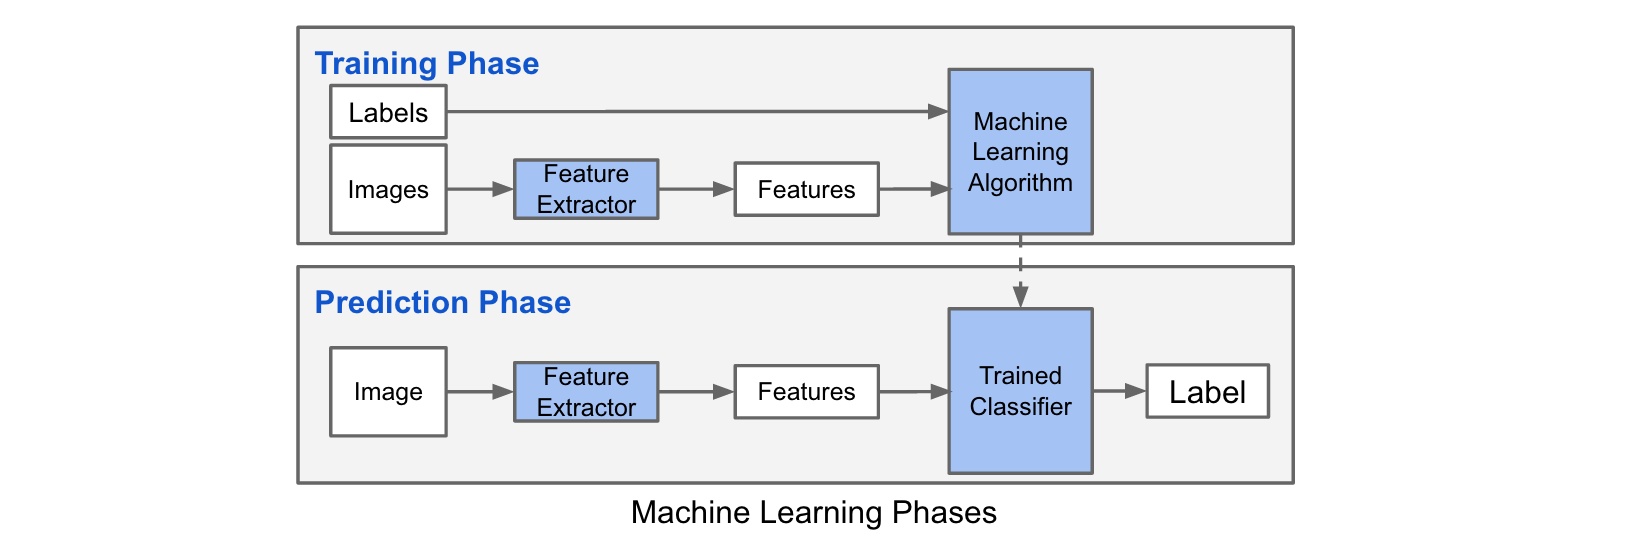
\includegraphics[width=\linewidth]{images/flow/generic.png}
	\caption{Generic flow for object recognition}
\end{figure}

\begin{figure}[h!]
	\centering
	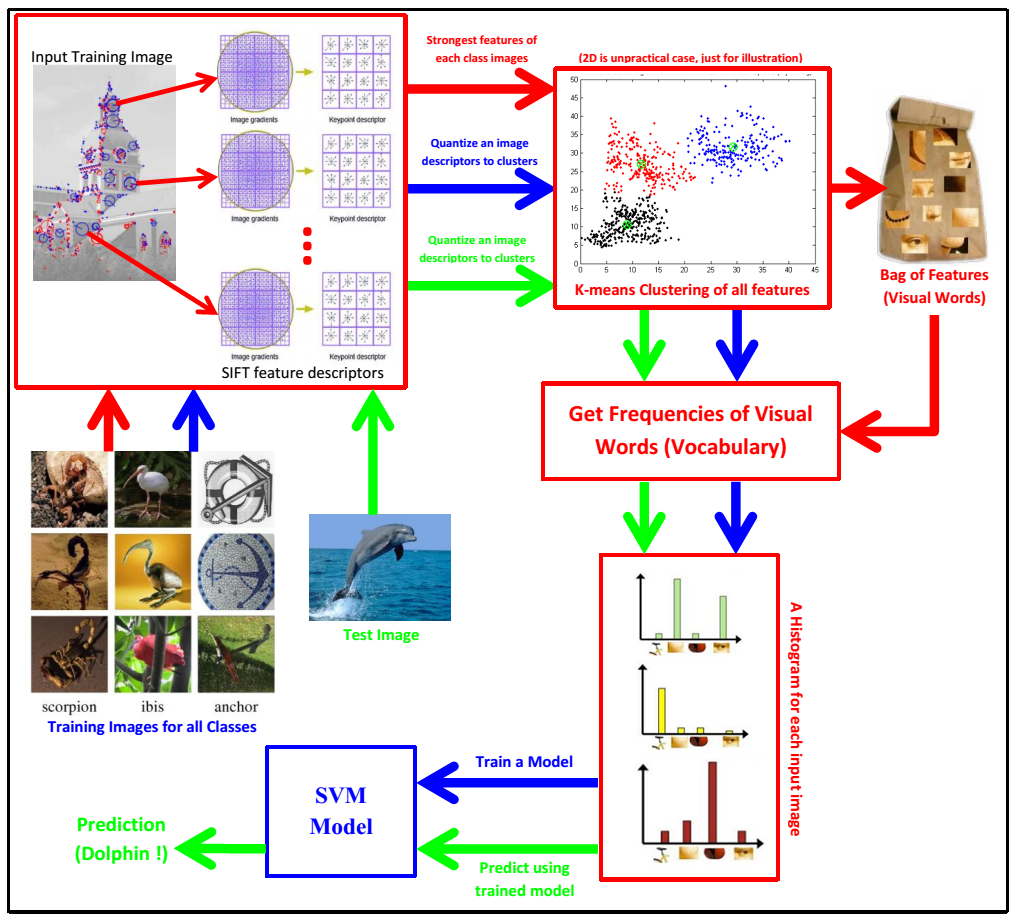
\includegraphics[width=0.8\linewidth]{images/flow/bow_svm.png}
	\caption[BOV-SVM flow chart]{The detail process of recognition with BOW and SVM}
\end{figure}

\subsection{Bag Of Visual Words (BOV)}
\subsubsection*{Over view}
The bag-of-words model is a \href{https://en.wikipedia.org/wiki/Vector_space_model}{\textcolor{blue}{vector space model}} representing text data when modeling text with machine learning algorithms. In practice, this model is mainly used as a tool of feature generation.

\subsubsection*{Basic idea}
\paragraph*{}
In doucment classification after transforming the text into a "bag of words", we can calculate various measures (also call features) to characterize the text. The most common type of characteristic is the histogram of words (based on the number of times a word appears in the document).

\paragraph*{}
In oder to use bag of words (from text) in computer vision (for images), we can treat image features as words. Thus, we have \textit{Bag Of Visual Words}. The vocabulary can be built up by clustering all feature points collected from a suitable source (Ex. the training set) with each cluster represents for a word. After we have the vocabulary, the histogram of words will be used as feature vector of an image.

\begin{figure}[h!]
	\centering
	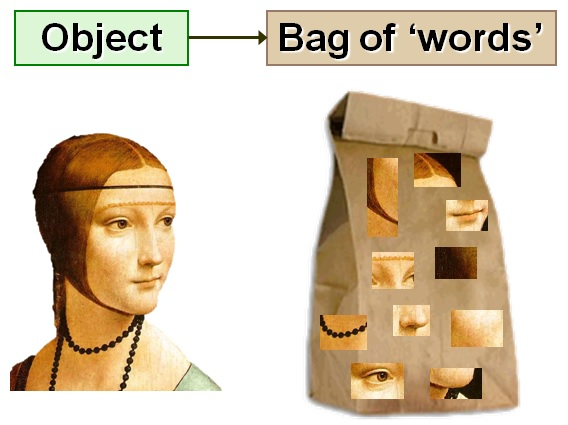
\includegraphics[width=0.6\linewidth]{images/bow/example.jpg}
	\caption[BOV example]{An example for BOV}
\end{figure}

\paragraph*{}
In this project, we use SIFT as feature extractor and K-Means as clustering algorithm to build the vocabulary.

\subsubsection*{Pseudo-code} 
\lstinputlisting{code/bow/create_vocabulary.txt}
\lstinputlisting{code/bow/cal_histogram.txt}
\lstinputlisting{code/bow/which_word.txt}

\subsection{K-Neareast Neighbor (KNN)}
\subsubsection*{Over view}
KNN is a type of \href{https://en.wikipedia.org/wiki/Instance-based_learning}{\textcolor{blue}{instance-based learning}}, or \href{https://en.wikipedia.org/wiki/Lazy_learning}{\textcolor{blue}{lazy learning}} which means we don't need to train a real model for redicting. 

\subsubsection*{Basic idea}
\paragraph*{}
The basic idea is with any unknown sample x (or a query point), finding k \textit{nearest samples} in training set and assigning the label which is most frequent among \textit{k-nearest samples} to that query point.

\begin{figure}[h!]
	\centering
	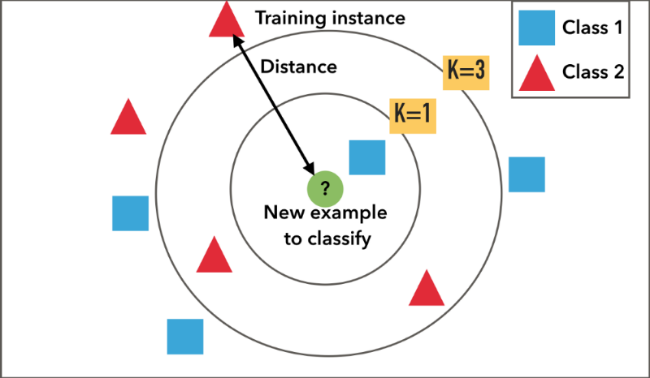
\includegraphics[width=0.8\linewidth]{images/knn/example.png}
	\caption[KNN example]{An example of KNN with different K}
\end{figure}

\paragraph*{}
A common method used for calculate the distance metric between samples is \href{https://en.wikipedia.org/wiki/Euclidean_distance}{\textcolor{blue}{Euclidean distance}}. We also use this model in this project for a simple implementation.

\subsubsection*{Pseudo-code}
\lstinputlisting{code/knn/knn.txt}

\subsection{Support Vector Machines (SVMs)}
\subsubsection*{Over view}
\paragraph*{}
SVMs are \href{https://en.wikipedia.org/wiki/Supervised_learning}{\textcolor{blue}{supervised learning}} models with associated learning algorithms that analyze data used for classification and regression analysis. \cite{WIKI:0}. In this project we only consider about classification.

\paragraph*{}
In 1957, a simple linear model called the Perceptron was invented by Frank Rosenblatt to do classification.

\paragraph*{}
A few years later,  Vapnik and Chervonenkis, proposed another model called the "Maximal Margin Classifier", the SVM was born.

\paragraph*{}
Then, in 1992, Vapnik et al. had the idea to apply what is called the Kernel Trick, which allow to use the SVM to classify linearly nonseparable data.

\paragraph*{}
Eventually, in 1995, Cortes and Vapnik introduced the Soft Margin Classifier which allows us to accept some misclassifications when using a SVM.

\paragraph*{}
So just when we talk about classification there is already four different Support Vector Machines:
\begin{enumerate}
\item The original one : the Maximal Margin Classifiers
\item The kernelized version using the Kernel Trick
\item The soft-margin version
\item The soft-margin kernelized version (which combine 1, 2 and 3)
\end{enumerate}

\paragraph*{}
For more detail about the history, you can read \href{http://www.svms.org/history.html}{\textcolor{blue}{here}}.

\paragraph*{}
In this project, we implement the last version for multi-classification with two approaches \textit{one vs one} and \textit{one vs rest} 

\subsubsection*{Basic idea}
In the case of SVM, it learns a linear model (a hyperplane) to seperate data. Let's take a quick look at how the first SVM (also call hard margin) is built up in simple case (linear sepratable data).
\paragraph*{} 
Before SVM, Perceptron Learning Algorithm is a simple model for finding a hyperplane to separate data. However, its biggest weakness is that it will not find the same hyperplane every time but not the best one (because of the randomness, you can find the detail \href{https://en.wikipedia.org/wiki/Perceptron}{\textcolor{blue}{here}}). SVMs solve this problem by finding the \textit{best hyperplane} (we call this the \textbf{optimal hyperplane}).

\begin{figure}[h!]
	\centering
	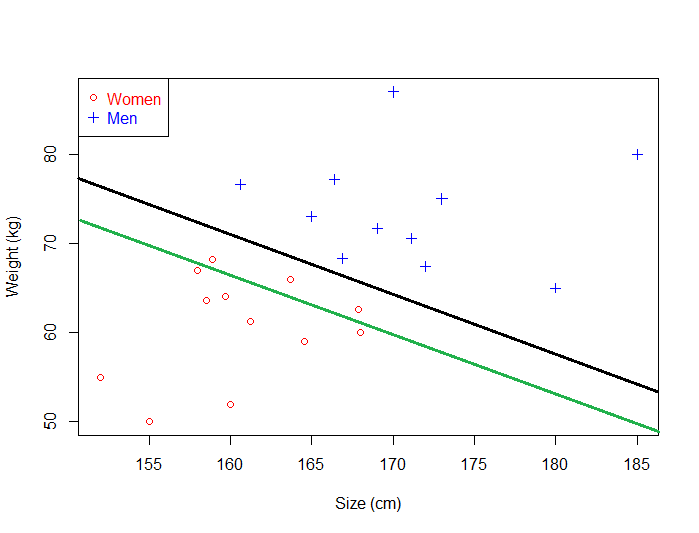
\includegraphics[width=\linewidth]{images/svm/compare_hyperplanes.png}
	\caption[Compare hyperplanes in SVMs]{The black hyperplane classifies more accurately than the green one}
\end{figure}

\paragraph*{}
SVMs compare two hyperplanes (which one is better for separate data) base on \textbf{the margin}.Basically the margin is a no man's land. There will never be any data point inside the margin. 

\paragraph*{}
We can make the following observations:
\begin{itemize}
	\item If an hyperplane is very close to a data point, its margin will be small.
	\item The further an hyperplane is from a data point, the larger its margin will be.
\end{itemize}
This means that the optimal hyperplane will be the one with the biggest margin.

\begin{figure}[h!]
	\centering
		\captionsetup{width=\textwidth}
	\centering
	\begin{subfigure}[b]{0.45\linewidth}
		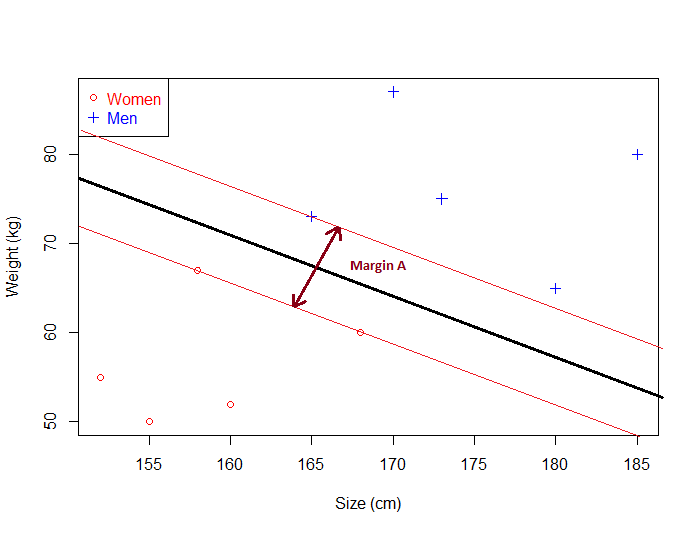
\includegraphics[width=\linewidth]{images/svm/margin0.png}
	\end{subfigure}
	\begin{subfigure}[b]{0.45\linewidth}
		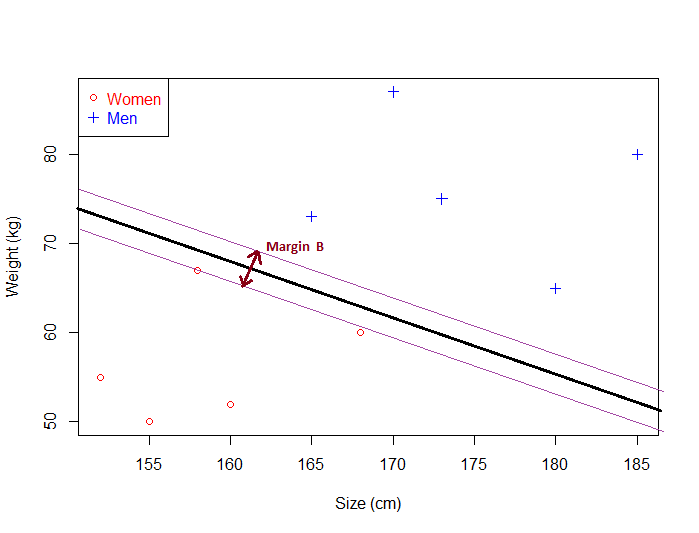
\includegraphics[width=\linewidth]{images/svm/margin1.png}
	\end{subfigure}
	\caption[The margin example]{Margin B is smaller than Margin A, so Margin A would be the better one for sperating data.}
\end{figure}

\paragraph*{}
In practice, we can compute the distance between the hyperplane and the closest data point. Once we have this value, if we double it we will the value of margin. After determine what the margin is and how to calculate it, we will solve the optimal problem (quadratic problem) to find the \textit{support vectors} and compute w, b parameter for the optiaml hyperplan from those \textit{support vector}.

\paragraph*{}
We will not go on the mathematics behind SVMs, but you can read \href{https://www.svm-tutorial.com/2017/10/support-vector-machines-succinctly-released/}{\textcolor{blue}{this book}}.

\subsubsection*{Pseudo-code}
For hard margin classification, all we need to do is let mathematis do the job (solve the quadratic problem). The quadratic problem solver we used is available here \href{http://cvxopt.org/}{\textcolor{blue}{scikit-learn libary}}. Below is an example code for using it.
\lstinputlisting{code/svm/hard_margin.txt}
For computing w
\lstinputlisting{code/svm/compute_w.txt}
For computing b
\lstinputlisting{code/svm/compute_b.txt}

